% Options for packages loaded elsewhere
\PassOptionsToPackage{unicode}{hyperref}
\PassOptionsToPackage{hyphens}{url}
%
\documentclass[
  ignorenonframetext,
]{beamer}
\usepackage{pgfpages}
\setbeamertemplate{caption}[numbered]
\setbeamertemplate{caption label separator}{: }
\setbeamercolor{caption name}{fg=normal text.fg}
\beamertemplatenavigationsymbolsempty
% Prevent slide breaks in the middle of a paragraph
\widowpenalties 1 10000
\raggedbottom
\setbeamertemplate{part page}{
  \centering
  \begin{beamercolorbox}[sep=16pt,center]{part title}
    \usebeamerfont{part title}\insertpart\par
  \end{beamercolorbox}
}
\setbeamertemplate{section page}{
  \centering
  \begin{beamercolorbox}[sep=12pt,center]{part title}
    \usebeamerfont{section title}\insertsection\par
  \end{beamercolorbox}
}
\setbeamertemplate{subsection page}{
  \centering
  \begin{beamercolorbox}[sep=8pt,center]{part title}
    \usebeamerfont{subsection title}\insertsubsection\par
  \end{beamercolorbox}
}
\AtBeginPart{
  \frame{\partpage}
}
\AtBeginSection{
  \ifbibliography
  \else
    \frame{\sectionpage}
  \fi
}
\AtBeginSubsection{
  \frame{\subsectionpage}
}
\usepackage{amsmath,amssymb}
\usepackage{lmodern}
\usepackage{ifxetex,ifluatex}
\ifnum 0\ifxetex 1\fi\ifluatex 1\fi=0 % if pdftex
  \usepackage[T1]{fontenc}
  \usepackage[utf8]{inputenc}
  \usepackage{textcomp} % provide euro and other symbols
\else % if luatex or xetex
  \usepackage{unicode-math}
  \defaultfontfeatures{Scale=MatchLowercase}
  \defaultfontfeatures[\rmfamily]{Ligatures=TeX,Scale=1}
  \setmainfont[BoldFont = SF Pro Rounded Semibold]{SF Pro Rounded}
  \setmathfont[]{STIX Two Math}
\fi
\usefonttheme{serif} % use mainfont rather than sansfont for slide text
% Use upquote if available, for straight quotes in verbatim environments
\IfFileExists{upquote.sty}{\usepackage{upquote}}{}
\IfFileExists{microtype.sty}{% use microtype if available
  \usepackage[]{microtype}
  \UseMicrotypeSet[protrusion]{basicmath} % disable protrusion for tt fonts
}{}
\makeatletter
\@ifundefined{KOMAClassName}{% if non-KOMA class
  \IfFileExists{parskip.sty}{%
    \usepackage{parskip}
  }{% else
    \setlength{\parindent}{0pt}
    \setlength{\parskip}{6pt plus 2pt minus 1pt}}
}{% if KOMA class
  \KOMAoptions{parskip=half}}
\makeatother
\usepackage{xcolor}
\IfFileExists{xurl.sty}{\usepackage{xurl}}{} % add URL line breaks if available
\IfFileExists{bookmark.sty}{\usepackage{bookmark}}{\usepackage{hyperref}}
\hypersetup{
  pdftitle={444 Lecture 8.1 - Iterated Prisoners' Dilemma},
  pdfauthor={Brian Weatherson},
  hidelinks,
  pdfcreator={LaTeX via pandoc}}
\urlstyle{same} % disable monospaced font for URLs
\newif\ifbibliography
\usepackage{graphicx}
\makeatletter
\def\maxwidth{\ifdim\Gin@nat@width>\linewidth\linewidth\else\Gin@nat@width\fi}
\def\maxheight{\ifdim\Gin@nat@height>\textheight\textheight\else\Gin@nat@height\fi}
\makeatother
% Scale images if necessary, so that they will not overflow the page
% margins by default, and it is still possible to overwrite the defaults
% using explicit options in \includegraphics[width, height, ...]{}
\setkeys{Gin}{width=\maxwidth,height=\maxheight,keepaspectratio}
% Set default figure placement to htbp
\makeatletter
\def\fps@figure{htbp}
\makeatother
\setlength{\emergencystretch}{3em} % prevent overfull lines
\providecommand{\tightlist}{%
  \setlength{\itemsep}{0pt}\setlength{\parskip}{0pt}}
\setcounter{secnumdepth}{-\maxdimen} % remove section numbering
\let\Tiny=\tiny

 \setbeamertemplate{navigation symbols}{} 

% \usetheme{Madrid}
 \usetheme[numbering=none, progressbar=foot]{metropolis}
 \usecolortheme{wolverine}
 \usepackage{color}
 \usepackage{MnSymbol}
% \usepackage{movie15}

\usepackage{amssymb}% http://ctan.org/pkg/amssymb
\usepackage{pifont}% http://ctan.org/pkg/pifont
\newcommand{\cmark}{\ding{51}}%
\newcommand{\xmark}{\ding{55}}%

\DeclareSymbolFont{symbolsC}{U}{txsyc}{m}{n}
\DeclareMathSymbol{\boxright}{\mathrel}{symbolsC}{128}
\DeclareMathAlphabet{\mathpzc}{OT1}{pzc}{m}{it}

\setlength{\parskip}{1ex plus 0.5ex minus 0.2ex}

\AtBeginSection[]
{
\begin{frame}
	\Huge{\color{darkblue} \insertsection}
\end{frame}
}

\renewenvironment*{quote}	
	{\list{}{\rightmargin   \leftmargin} \item } 	
	{\endlist }

\definecolor{darkgreen}{rgb}{0,0.7,0}
\definecolor{darkblue}{rgb}{0,0,0.8}

\usepackage[italic]{mathastext}
\usepackage{nicefrac}
\usepackage{istgame}

\setbeamertemplate{caption}{\raggedright\insertcaption}

%\def\toprule{}
%\def\bottomrule{}
%\def\midrule{}
\usepackage{etoolbox}
\AfterEndEnvironment{description}{\vspace{9pt}}
\AfterEndEnvironment{oltableau}{\vspace{9pt}}
\BeforeBeginEnvironment{oltableau}{\vspace{9pt}}
\AfterEndEnvironment{center}{\vspace{9pt}}
\BeforeBeginEnvironment{tabular}{\vspace{9pt}}
\AfterEndEnvironment{longtable}{\vspace{-6pt}}
\usepackage{booktabs}
\usepackage{longtable}
\usepackage{array}
\usepackage{multirow}
\usepackage{wrapfig}
\usepackage{float}
\usepackage{colortbl}
\usepackage{pdflscape}
\usepackage{tabu}
\usepackage{threeparttable} 
\usepackage{threeparttablex} 
\usepackage[normalem]{ulem} 
\usepackage{makecell}
\usepackage{xcolor}
\usepackage{ulem}

\setlength\heavyrulewidth{0ex}
\setlength\lightrulewidth{0.08ex}

\aboverulesep=0ex
\belowrulesep=0ex
\renewcommand{\arraystretch}{1.2}
\ifluatex
  \usepackage{selnolig}  % disable illegal ligatures
\fi

\title{444 Lecture 8.1 - Iterated Prisoners' Dilemma}
\author{Brian Weatherson}
\date{}

\begin{document}
\frame{\titlepage}

\begin{frame}{Prisoners' Dilemma}
\protect\hypertarget{prisoners-dilemma}{}
Basic Challenge:

\begin{itemize}
\tightlist
\item
  Each player is better off defecting;
\item
  The players are collectively better off if both cooperate.
\end{itemize}
\end{frame}

\begin{frame}{Tragedy of the Commons}
\protect\hypertarget{tragedy-of-the-commons}{}
\begin{itemize}
\tightlist
\item
  In a two-player setting, we normally call this Prisoners' Dilemma, or
  PD.
\item
  In a multi-player setting it's sometimes called the Tragedy of the
  Commons.
\item
  The story (which may be wildly ahistorical) is that everyone grazed
  their herds on the commons - which was a good thing to do or else the
  herd would die - but collectively this made the commons unusable.
\item
  And in the standard story, private property was the solution to the
  tragedy.
\end{itemize}
\end{frame}

\begin{frame}{Social Challenge}
\protect\hypertarget{social-challenge}{}
\begin{itemize}[<+->]
\tightlist
\item
  How do we get to cooperation?
\item
  First question is whether in this case we should want to get to
  cooperation.
\item
  Second question is whether this really is PD.
\item
  Let's assume that the answer in each case is \emph{yes}, what do we
  do.
\end{itemize}
\end{frame}

\begin{frame}{Change the Payouts}
\protect\hypertarget{change-the-payouts}{}
One possible social response is to change the payouts.

\begin{itemize}
\tightlist
\item
  \emph{Snitches get stiches} is kind of a version of this response.
\end{itemize}
\end{frame}

\begin{frame}{Change the Options}
\protect\hypertarget{change-the-options}{}
Another is to make it just impossible for everyone to do the defecting
move.

\begin{itemize}
\tightlist
\item
  Enclosures are sort of like this.
\item
  Just like with signaling games, the difference between making
  something expensive and making it impossible is a little vague, but
  it's useful conceptually to think of them as separate options.
\end{itemize}
\end{frame}

\begin{frame}{Iterate the Game}
\protect\hypertarget{iterate-the-game}{}
\begin{itemize}
\tightlist
\item
  But the simplest way to handle this kind of problem is to iterate the
  game.
\item
  Arguably it is in everyone's interests to be cooperative if they will
  have to interact with the other players repeatedly.
\end{itemize}
\end{frame}

\begin{frame}{Robert Axelrod}
\protect\hypertarget{robert-axelrod}{}
\begin{figure}
\centering
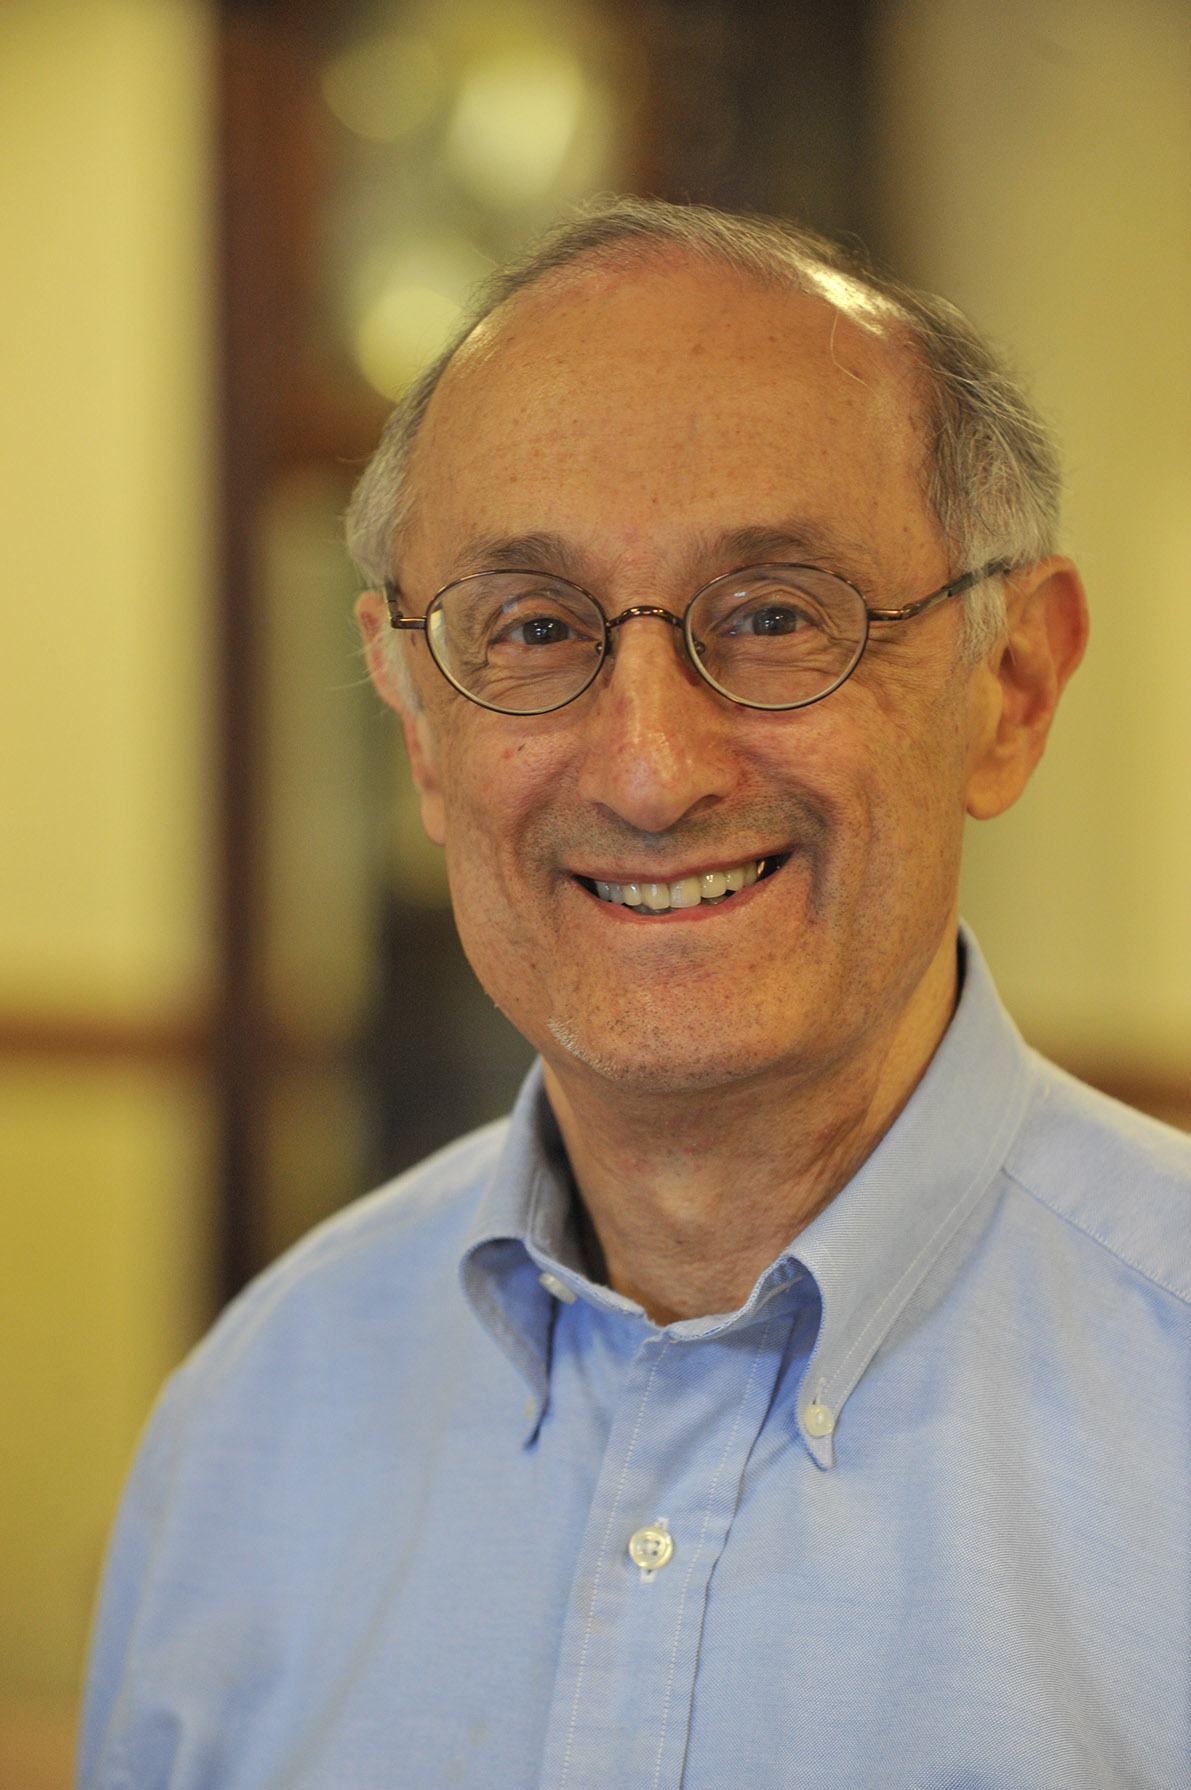
\includegraphics[width=\textwidth,height=0.8\textheight]{Axelrod.jpg}
\caption{Robert Axelrod}
\end{figure}
\end{frame}

\begin{frame}{The Evolution of Cooperation}
\protect\hypertarget{the-evolution-of-cooperation}{}
\begin{figure}
\centering
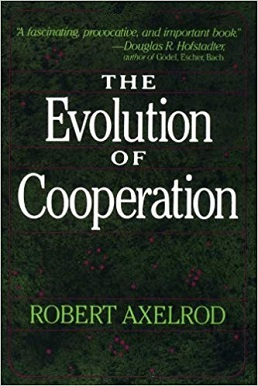
\includegraphics{The_Evolution_of_Cooperation.jpg}
\caption{Axelrod's Famous 1984 Book}
\end{figure}
\end{frame}

\begin{frame}{The One Shot Game}
\protect\hypertarget{the-one-shot-game}{}
Axelrod worked with this version of Prisoners' Dilemma (PD).

\begin{table}[!h]
\centering
\begin{tabular}[t]{>{}r|cc}
\toprule
 & c & d\\
\midrule
C & 3, 3 & 0, 5\\
D & 5, 0 & 1, 1\\
\bottomrule
\end{tabular}
\end{table}
\end{frame}

\begin{frame}{Indefinite Iteration}
\protect\hypertarget{indefinite-iteration}{}
In the fancier version of the game, he didn't tell people how long the
game would go.

\begin{itemize}
\tightlist
\item
  Instead he just said there was a probability of it ending after each
  round; if I recall 0.005.
\item
  This was used to avoid backwards induction reasoning.
\item
  It turned out not to really mater a ton; no one uses backward
  induction reasoning in practice. But it's theoretically useful.
\end{itemize}
\end{frame}

\begin{frame}{The Tournament}
\protect\hypertarget{the-tournament}{}
\begin{itemize}
\tightlist
\item
  There are \emph{n} strategies submitted.
\item
  Strategies are not quite full strategies in our sense; they just say
  what to do given what the other player did. (They don't account for
  possible errors in their own performance.)
\item
  Each will play \emph{k} rounds of PD with each of the other \emph{n}-1
  strategies.
\item
  Their payouts will add up over the \(k(n-1)\) rounds and the one with
  the highest total will win.
\end{itemize}
\end{frame}

\begin{frame}{Cooperative and Competitive}
\protect\hypertarget{cooperative-and-competitive}{}
\begin{itemize}
\tightlist
\item
  This is not entirely a cooperative game; ultimately if I'm a strategy
  I want to win, and that means I want the other strategy I'm
  interaction with to lose.
\item
  But in the short run there is much to be gained by improving our
  mutual position vs the other \(n-2\) strategies.
\item
  So in the short run there is a benefit to cooperation, even if we're
  ultimately rivals.
\end{itemize}
\end{frame}

\begin{frame}{Iterated Axelrod Game}
\protect\hypertarget{iterated-axelrod-game}{}
\begin{itemize}
\tightlist
\item
  Axelrod famously ran a tournament just like the one described here.
\item
  But we can iterate the whole tournament in an interesting way.
\item
  Imagine at the start each strategy is \(1/n\) of the overall
  `population'.
\item
  After playing all these games, where each strategy plays \(k(n-1)\)
  versions of PD, each strategy gets a score.
\item
  In the next round, it's share of the population is a function of (a)
  its initial population, and (b) its score in this round.
\item
  And in future rounds, one's score is a weighted average of how well
  one does in games against the other strategies, where the weights are
  given by their populations.
\end{itemize}
\end{frame}

\begin{frame}{Evolution of Cooperation}
\protect\hypertarget{evolution-of-cooperation}{}
\begin{itemize}
\tightlist
\item
  This is a useful model for thinking about the phenomena in the title
  of Axelrod's book: The Evolution of Cooperation.
\item
  We want strategies that do well not just when the world consists of
  random strategies, but when the world consists of strategies that
  themselves could have survived at least a little bit of evolution.
\item
  At a big picture level this doesn't change a lot about what does well
  in Iterated PD, but theoretically it could make a difference.
\item
  Strategies that exploit dumb strategies could do well initially, but
  then fade away.
\item
  Alternatively, some strategies could do badly against bad strategies,
  but if they survive initial rounds, do well when there are
  sophisticated strategies around.
\end{itemize}
\end{frame}

\begin{frame}{Spatial Evolution}
\protect\hypertarget{spatial-evolution}{}
\begin{itemize}
\tightlist
\item
  To be even more realistic, you could imagine that each strategy lives
  `somewhere' in a large grid.
\item
  And at each round, each strategy plays with a weighted average of
  strategies that live nearby.
\item
  This really does make a difference; some strategies that aren't great
  against the world in general are fairly immune to invasion, and can
  even expand their territory under a range of conditions.
\end{itemize}
\end{frame}

\begin{frame}{For Next Time}
\protect\hypertarget{for-next-time}{}
We'll go over the results of the Axelrod tournaments.
\end{frame}

\end{document}
